\documentclass[12pt,a4paper]{article}
\usepackage[a4paper,total={160mm,250mm}]{geometry}
\usepackage[utf8]{inputenc}
\usepackage[ruled,vlined]{algorithm2e}
\usepackage{amsmath}
\usepackage{amsthm}
\usepackage{amsfonts}
\usepackage{amssymb}
\usepackage{amscd}
\usepackage{array}
\usepackage{caption}
\usepackage{dirtree}
\usepackage{enumitem}
\usepackage{graphicx}
\usepackage{hyperref}
\usepackage{listings}
\usepackage{mathtools}
\usepackage{ngerman}
\usepackage{subcaption}
\usepackage{tcolorbox}
\usepackage{tikz}
\usepackage{xcolor}

\definecolor{shade}{gray}{.5}

\renewcommand{\thesubfigure}{\roman{subfigure}}

\theoremstyle{definition}
\newtheorem{aufgabe}{Aufgabe}

\theoremstyle{definition}
\newtheorem*{losung*}{Lösung}

\theoremstyle{definition}
\newtheorem*{beispiel*}{Beispiel}

\definecolor{mygreen}{rgb}{0,0.6,0}
\definecolor{mygray}{rgb}{0.5,0.5,0.5}
\definecolor{mymauve}{rgb}{0.58,0,0.82}
\definecolor{lightgray}{rgb}{0.9,0.9,0.9}

\lstset{inputpath=../raytracer}
\lstdefinestyle{python}{
	backgroundcolor=\color{lightgray},   % choose the background color; you must add \usepackage{color} or \usepackage{xcolor}; should come as last argument
	basicstyle=\footnotesize\ttfamily,        % the size of the fonts that are used for the code
	breakatwhitespace=false,         % sets if automatic breaks should only happen at whitespace
	breaklines=true,                 % sets automatic line breaking
	captionpos=b,                    % sets the caption-position to bottom
	commentstyle=\color{mygreen},    % comment style
	deletekeywords={...},            % if you want to delete keywords from the given language
	escapeinside={\\[}{\\]},          % if you want to add LaTeX within your code
	extendedchars=true,              % lets you use non-ASCII characters; for 8-bits encodings only, does not work with UTF-8
	firstnumber=1,                   % start line enumeration with line 1000
	frame=single,	                 % adds a frame around the code
	keepspaces=true,                 % keeps spaces in text, useful for keeping indentation of code (possibly needs columns=flexible)
	keywordstyle=\color{blue},       % keyword style
	language=Python,                 % the language of the code
	literate=%
	    {ä}{{\"a}}1%
		{ö}{{\"o}}1%
		{ü}{{\"u}}1%
		{ß}{{\ss}}1%
		{Ä}{{\"A}}1%
		{Ö}{{\"O}}1%
		{Ü}{{\"U}}1,%
	morekeywords={*,...},            % if you want to add more keywords to the set
	numbers=left,                    % where to put the line-numbers; possible values are (none, left, right)
	numbersep=5pt,                   % how far the line-numbers are from the code
	numberstyle=\tiny\color{mygray}, % the style that is used for the line-numbers
	rulecolor=\color{black},         % if not set, the frame-color may be changed on line-breaks within not-black text (e.g. comments (green here))
	showspaces=false,                % show spaces everywhere adding particular underscores; it overrides 'showstringspaces'
	showstringspaces=false,          % underline spaces within strings only
	showtabs=false,                  % show tabs within strings adding particular underscores
	stepnumber=1,                    % the step between two line-numbers. If it's 1, each line will be numbered
	stringstyle=\color{mymauve},     % string literal style
	tabsize=4,	                     % sets default tabsize to 2 spaces
	title=\lstname,                   % show the filename of files included with \lstinputlisting; also try caption instead of title
	rangeprefix=\#---,
	rangesuffix=---,
	includerangemarker=false
}

%\pagestyle{empty}

\title{Eigengesichter}
\author{Oliver Rietmann}
\date{\today}

\begin{document}
\begin{titlepage}
	{\hspace{-1cm}
\includegraphics[width=0.3\textwidth]{images/ETHlogo}\par}
	\vspace{1cm}
	\begin{center}
	{\scshape Mentorierte Arbeit in Fachdidaktik Mathematik\par}
	\vspace{1cm}
	{\large\bfseries Eigengesichter\par}
	\vspace{1cm}
	{Oliver Rietmann\par}
	\vfill
	\end{center}
	{\bfseries Inhalt\par}
	{In dieser Arbeit wird die Technik der \textit{Eigengesichter} (engl. \textit{eigenfaces}) erklärt. Hierbei handelt es sich um eine eine rudimentäre Methode zur Gesichtserkennung, welche durch Computer automatisiert werden kann. Unter Gesichtserkennung versteht man klassischerweise das (automatisierte) identifizieren einer Person auf einem Foto. Aber auch damit verwandte Aufgaben werden hier besprochen.
	Diese Arbeit führt die Leser durch eine Anleitung zur Implementierung eines solchen Programms in Python. Der Fokus liegt dabei auf der zugrundeliegenden Mathematik dieses Verfahrens. Die dazu verwendeten Unterrichtsmethoden sollen zudem aus didaktischer Sicht beleuchtet werden.\par}
	\vspace{0.5cm}
	{\bfseries Zielpublikum\par}
	{Fortgeschrittene gymnasiale Mittelschüler mit Schwerpunkt Mathematik und Studenten einer mathematischen/technischer Fachrichtung.\par}
	\vspace{0.5cm}
	{\bfseries Voraussetzungen\par}
	{Vertrautheit mit den Grundbegriffen der linearen Algebra (Vektoren, Matrizen, Basis, Linearkombination, Unterräume von $\mathbb R^n$).
	Zudem werden grundlegende Programmierkenntnisse vorausgesetzt.\par}
	\vspace{0.5cm}
	{\bfseries Form\par}
	{Text mit Aufgaben, Lösungen und Lernzielen. Die Python-Codes befinden sich im Anhang. Alternativ können sie online heruntergeladen werden. (Der Link befindet sich in der Arbeit.)\par}
	\vspace{0.5cm}
	{\bfseries Betreuung\par}
	{Christian Rüede\par}
	\vspace{0.5cm}
	{\bfseries Datum\par}
	{\today\par}
\end{titlepage}
%\maketitle
%\tableofcontents
\clearpage
\section*{Einleitung}
Historisch gesehen war die Methode der Eigengesichter das erste durch Computer automatisierbare Verfahren zur Gesichtserkennung.
Das Fundament dazu wurde 1987 durch Sirovich and Kirby entwickelt \cite{SirovichKirby1987}.
In ihrer Arbeit verwendeten Sie bereits den Begriff \textit{eigenpictures}.
Sie zeigten auf, wie man Fotos von Gesichtern geeignet durch Begriffe der linearen Algebra beschreiben kann.
Damit war der Weg frei um die mächtige Maschinerie der Mathematik, insbesondere der linearen Algebra und der Statistik, auf Fotos anzuwenden.
Dies geschah schon kurz darauf, nämlich 1991, durch Turk und Pentland \cite{Turk1991}.
Sie verwendeten bereits den Begriff \textit{eigenfaces} und beschrieben das Verfahren zur Gesichtserkennung, welches auch wir implementieren werden.
Modernere Methoden wie zum Beispiel \textit{DeepFace} von Facebook funktionieren allerdings viel besser als unsere rudimentäre Methode und sind so gut wie echte Menschen bei der Gesichtserkennung \cite{Taigman2014}.
Ein Vergleich der (heutzutage) besten Methoden findet man zum Beispiel hier \cite{Taskiran2020}.

Alle solchen Programme, auch die modernsten, verwenden eine \textit{Datenbank} von Bildern von Gesichtern, deren Identität bereits bekannt ist.
Man hat also eine gewisse Anzahl von Personen.
Jeder einzelnen Person sind mehrere Bilder zugeordnet, nämlich die Bilder, welche das Gesicht eben dieser Person zeigen.
Man kann sich das als Unterteilung in verschiedene Klassen vorstellen: Zu jeder Person gehört eine Klasse und jede Klasse enthält eine Menge von Bildern.
Dies ist in Abbildung~\ref{fig:database} veranschaulicht.
\begin{figure}[ht]
	\centering
	\begin{tabular}{l m{2cm} m{2cm} m{2cm} m{2cm} c}
		\textbf{Klasse (Person)} & \textbf{Bild 1} & \textbf{Bild 2} & \textbf{Bild 3} & \textbf{Bild 4} & $\cdots$ \\ \hline
		Adam Sandler & 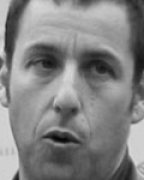
\includegraphics[width=0.1\textwidth]{images/intro/class0_0} &
		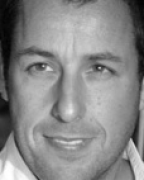
\includegraphics[width=0.1\textwidth]{images/intro/class0_1} & 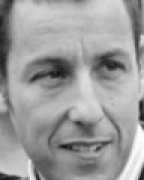
\includegraphics[width=0.1\textwidth]{images/intro/class0_2} & 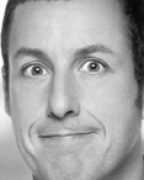
\includegraphics[width=0.1\textwidth]{images/intro/class0_3} & $\cdots$ \\ \hline
		Emma Watson & 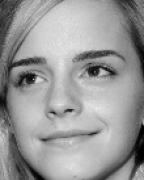
\includegraphics[width=0.1\textwidth]{images/intro/class1_0} &
		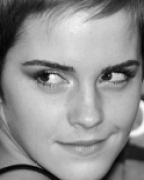
\includegraphics[width=0.1\textwidth]{images/intro/class1_1} & 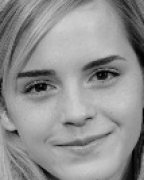
\includegraphics[width=0.1\textwidth]{images/intro/class1_2} & 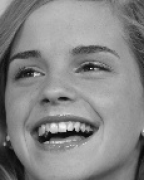
\includegraphics[width=0.1\textwidth]{images/intro/class1_3} & $\cdots$ \\ \hline
		Natalie Portman & 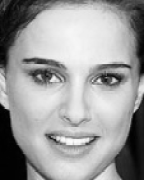
\includegraphics[width=0.1\textwidth]{images/intro/class2_0} & 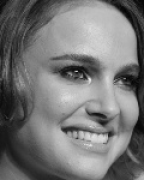
\includegraphics[width=0.1\textwidth]{images/intro/class2_1} & 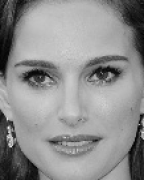
\includegraphics[width=0.1\textwidth]{images/intro/class2_2} & 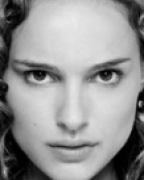
\includegraphics[width=0.1\textwidth]{images/intro/class2_3} & $\cdots$ \\ \hline
		$\qquad\qquad\vdots$ & $\qquad\vdots$ & $\qquad\vdots$ & $\qquad\vdots$ & $\qquad\vdots$ & $\ddots$ \\
	\end{tabular}
	\caption{Visualisierng einer Datenbank von Bildern von Gesichtern.}
	\label{fig:database}
\end{figure}
Aus dieser Datenbank \glqq{}lernt\grqq{} das Programm, neue Bilder zu klassifizieren, also den Personen aus der Datenbank zuzuordnen.
Das Wort \glqq{}neu\grqq{} bedeutet hier, dass dieses Bild nicht notwendigerweise in der Datenbank enthalten ist.
Die Person auf dem Bild muss aber in der Datenbank sein!
Würde die Datenbank in Abbildung~\ref{fig:database} wirklich nur diese drei Personen enthalten, so könnte man zum Beispiel kein Bild von Brad Pitt korrekt klassifizieren, auch wenn eine noch so gute Methode verwendet wird.
Die Datenbank und die Methode der Gesichtserkennung sind unabhängig voneinander.
Das heisst einerseits, aus der selben Datenbank können verschiedene Methoden lernen.
Andererseits kann ein und die selbe Methode verschiedene Datenbanken nutzen.
Wie gut die Gesichtserkennung am Schluss funktioniert hängt nicht nur von der Methode selbst ab, sondern auch von der Datenbank, welche diese verwendet.
Grundsätzlich gilt, dass jede Methode umso besser funktioniert, je mehr Bilder pro Person in der Datenbank gespeichert sind, die sie verwendet.
Mit \glqq{}gut funktionieren\grqq{} ist gemeint, dass neue Bilder mit hoher Wahrscheinlichkeit richtig klassifiziert werden.

Die in Abbildung~\ref{fig:database} gezeigten Bilder stammen aus einer Datenbank von über 10'000 Bildern von über 100 berühmten Persönlichkeiten \cite{Chen14}.
Die Bilder sind alle schwarz-weiss und zeigen lediglich die Gesichter der Personen.
Genau diese Datenbank werden wir auch für alle nachfolgenden Kapitel verwenden \textcolor{green}{(Link zur Datenbank folgt)}.
Allerdings kann auch eine andere Datenbank verwendet werden, sofern sie in das richtige Format gebracht wird \textcolor{green}{(Kapitel dazu folgt)}.

Das Grundgerüst eines Programms zur Gesichtserkennung in Python steht uns schon zur Verfügung.
Wir werden dieses in den folgenden Kapiteln zu einem voll funktionsfähigen Programm erweitern.
Der gesamte Code befindet sich im Anhang \textcolor{green}{(folgt)} und kann unter folgendem Link heruntergeladen werden \textcolor{green}{(Link zum Code folgt)}.
%\section{Eigengesichter}
In diesem Kapitel werden wir sehen was die Eigengesichter eigentlich sind.
Zu einer gegebenen Datenbank werden wir diese berechnen und mit unserem Python Code visualisieren.
Allerdings werden wir noch noch keine Gesichtserkennung vornehmen.
\begin{tcolorbox}
	\centerline{\textbf{Lernziele Kapitel 1}}
	\begin{enumerate}[leftmargin=*]
		\item Darstellung eines schwarz-weiss Bildes als Vektor \textit{verstehen}.
		\item Die Begriffe Durchschnittsgesicht, Differenzgesicht und Eigengesicht \textit{verstehen}.
		\item Die Singulärwertzerlegung als Blackbox \textit{anwenden} können.
	\end{enumerate}
\end{tcolorbox}
\section{Vom Bild zum Vektor} \label{sec:vectormatrix}
\begin{tcolorbox}
	\centerline{\textbf{Lernziele Kapitel~\ref{sec:vectormatrix}}}
	\begin{enumerate}[leftmargin=*]
		\item Darstellung eines schwarz-weiss Bildes als Vektor \textit{verstehen}.
		\item Die grundlegenden Matrix und Vektor Operation in Python \textit{anwenden} können (Addition, Multiplikation, Einträge auslesen oder verändern).
	\end{enumerate}
\end{tcolorbox}
Der erste Schritt besteht darin, Bilder als Vektoren aufzufassen.
Das hat zwei Gründe: Erstens können wir diese nur so geeignet in Python darstellen und manipulieren.
Zweitens erlaubt uns das, Bilder in den Kontext der linearen Algebra zu bringen um deren mächtige Methoden anzuwenden.
Als Beispiel betrachten wir ein Bild der Auflösung $N=144$ Pixel (Breite) mal $M=180$ Pixel (Höhe), wie in Abbildung~\ref{fig:image_to_vector}.
Jedem Pixel wird nun eine reelle Zahl zwischen Null und Eins zugeordnet.
Nehmen wir das Pixel an der Stelle $\left(i,j\right)\in\mathbb N^M\times\mathbb N^N$.
Zum Beispiel entspricht $\left(1,N\right)$ dem Pixel in der oberen rechten Ecke des Bildes.
Diesem Pixel wird also eine Zahl $p_{ij}\in\left[0,1\right]$ zugeordnet.
Dabei bedeutet $p_{ij}=0$, dass das Pixel schwarz ist und $p_{ij}=1$, dass es weiss ist.
Die Zahlen dazwischen entsprechen den Graustufen.
Das gibt uns eine $N\times M$-Matrix deren Einträge gerade die $p_{ij}$ sind.
So können wir also ein schwarz-weiss Bild als Matrix auffassen.
Nun schreiben wir die Spalten dieser Matrix in einen Vektor wie in Abbildung~\ref{fig:image_to_vector} gezeigt.
Mit dieser Abbildungsvorschrift können wir jedem schwarz-weiss Bild der Auflösung $N\times M$ auf eindeutige Weise einen Vektor in $\left[0,1\right]^{N\cdot M}$ zuordnen.
Jeder solche Vektor lässt sich auch wieder als Bild darstellen.
Für diesen Schritt ist es egal ob das Bild ein Gesicht zeigt oder etwas anderes.
\begin{figure}[ht]
	\centering
	\begin{tabular}{m{3.5cm} m{1cm} c m{1cm} c}
		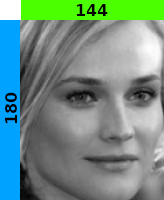
\includegraphics[width=0.2\textwidth]{images/vectormatrix/ImageToVector} &
		$\longrightarrow$ &
		$\begin{pmatrix}
			\textcolor{violet}{p_{11}} & \textcolor{orange}{p_{12}} & \cdots & \textcolor{olive}{p_{1N}} \\
			\textcolor{violet}{\vdots} & \textcolor{orange}{\vdots} & \ddots & \textcolor{olive}{\vdots} \\
			\textcolor{violet}{p_{M1}} & \textcolor{orange}{p_{M2}} & \cdots &  \textcolor{olive}{p_{MN}} \\
		\end{pmatrix}$ &
		$\longrightarrow$ &
		$\begin{pmatrix}
			\textcolor{violet}{p_{11}} \\
			\textcolor{violet}{\vdots} \\
			\textcolor{violet}{p_{M1}} \\
			\textcolor{orange}{p_{12}} \\
			\textcolor{orange}{\vdots} \\
			\textcolor{orange}{p_{M2}} \\
			\vdots \\
			\textcolor{olive}{p_{1N}} \\
			\textcolor{olive}{\vdots} \\
			\textcolor{olive}{p_{MN}} \\
		\end{pmatrix}$
	\end{tabular}
	\caption{Ein schwarz-weiss Bild kann als Matrix oder Vektor aufgefasst werden.}
	\label{fig:image_to_vector}
\end{figure}
\pagebreak[4]
\begin{aufgabe}
	Man betrachte das schwarz-weiss Bild, welches durch folgende Matrix beschrieben ist.
	\begin{equation*}
		\begin{pmatrix}
			1 & \frac{1}{4} \\
			\frac{1}{2} & 0 \\
			0 & \frac{3}{4} \\
		\end{pmatrix}
	\end{equation*}
	\begin{enumerate}[label=(\alph*)]
		\item Welche Werte für $N$ und $M$ beschreiben die Auflösung dieses Bildes?
		\item Wie sieht der Vektor aus, der dieses Bild beschreibt?
		\item Welches der folgenden drei Bilder entspricht dieser Matrix?
		
		\definecolor{onefourth}{rgb}{0.25, 0.25, 0.25}
		\definecolor{onehalf}{rgb}{0.5, 0.5, 0.5}
		\definecolor{threefourth}{rgb}{0.75, 0.75, 0.75}
		
		\qquad\qquad
		\begin{tikzpicture}
			\draw[step=1cm,white,very thin] (0,0) grid (2,3);
			\fill[white] (0,0) rectangle (1,1);
			\fill[onefourth] (1,0) rectangle (2,1);
			\fill[onehalf] (0,1) rectangle (1,2);
			\fill[white] (1,1) rectangle (2,2);
			\fill[black] (0,2) rectangle (1,3);
			\fill[threefourth] (1,2) rectangle (2,3);
		\end{tikzpicture}
		\qquad\qquad
		\begin{tikzpicture}
			\draw[step=1cm,white,very thin] (0,0) grid (2,3);
			\fill[black] (0,0) rectangle (1,1);
			\fill[threefourth] (1,0) rectangle (2,1);
			\fill[onehalf] (0,1) rectangle (1,2);
			\fill[black] (1,1) rectangle (2,2);
			\fill[white] (0,2) rectangle (1,3);
			\fill[onefourth] (1,2) rectangle (2,3);
		\end{tikzpicture}
		\qquad\qquad
		\begin{tikzpicture}
			\draw[step=1cm,white,very thin] (0,0) grid (2,3);
			\fill[black] (0,0) rectangle (1,1);
			\fill[onefourth] (1,0) rectangle (2,1);
			\fill[onehalf] (0,1) rectangle (1,2);
			\fill[black] (1,1) rectangle (2,2);
			\fill[white] (0,2) rectangle (1,3);
			\fill[threefourth] (1,2) rectangle (2,3);
		\end{tikzpicture}
	\end{enumerate}
\end{aufgabe}
\begin{losung*}
	Die Lösung der ersten beiden Teilaufgaben kann von Abbildung~\ref{fig:image_to_vector} abgelesen werden.
	Für die letzte Teilaufgabe erinnern wir uns, dass die Zahlen in $\left[0,1\right]$ fliessend den Graustufen von Schwarz (Null) bis Weiss (Eins) entsprechen.
	\begin{enumerate}[label=(\alph*)]
		\item Die Auflösung ist $N=3$ mal $M=2$ Pixel.
		\item Der Vektor ist gegeben durch
		\begin{equation*}
			\begin{pmatrix}
				1 \\
				\frac{1}{2} \\
				0 \\
				\frac{1}{4} \\
				0 \\
				\frac{3}{4} \\
			\end{pmatrix}.
		\end{equation*}
		\item Das mittlere Bild entspricht der Matrix.
	\end{enumerate}
\end{losung*}
In unserem Python Code ist die Funktion, welche eine $N\times M$ Matrix auf diese Weise in einen Vektor der Länge $N\cdot M$ überführt, bereits implementiert.
Sie befindet sich im File \texttt{eigenfaces.py} und heisst \texttt{matrix\_to\_vector}.
Wir betrachten diese nun etwas genauer, um die Manipulation von Matrizen und Vektoren in Python zu lernen.
\begin{lstlisting}[style=python]
import numpy as np

def matrix_to_vector(P, M, N):
	v = np.zeros(M * N)
	for i in range(M):
		for j in range(N):
			v[j + N * i] = P[i, j]
	return v
\end{lstlisting}
Das Argument \texttt{P} ist eine  \texttt{M} mal \texttt{N} Matrix und besteht aus den Einträgen $p_{ij}\in\left[0,1\right]$ wie oben.
Auf die Einträge von Vektoren und Matrizen kann über die eckigen Klammern $[$ und $]$ zugegriffen werden.
Wir brauchen aber auch die Umkehrung dieser Operation.
Das ist der Zweck folgender Übung.
\begin{aufgabe}
	Ergänzen Sie im File \texttt{eigenfaces.py} die Funktion \texttt{vector\_to\_matrix(v, M, N)}.
	Dabei ist \texttt{v} ein Vektor der Länge $\texttt{M}\cdot\texttt{N}$ wie oben.
	Die Funktion soll die zu \texttt{v} gehörende Matrix zurück geben.
	Sie können die ihre Lösung überprüfen indem Sie das Skript \texttt{vector\_to\_matrix\_test.py} laufen lassen.
\end{aufgabe}
\begin{losung*}
	Bei einer richtigen Lösung sollte das Skript \texttt{vector\_to\_matrix\_test.py} das Foto aus Abbildung~\ref{fig:image_to_vector} generieren.
	Die Lösung könnte zum Beispiel so aussehen:
\begin{lstlisting}[style=python]
import numpy as np

def vector_to_matrix(v, M, N):
	P = np.zeros(M, N)
	for i in range(M):
		for j in range(N):
			P[i, j] = v[j + N * i]
	return P
\end{lstlisting}
\end{losung*}
\subsection{Unterraum der Differenzgesichter}
Seien nun $M,N\in\mathbb N$ fix.
Wir haben im letzten Kapitel gesehen, wie man schwarz-weiss Bilder der Auflösung $M\times N$ als Vektoren in $\mathbb R^{M\cdot N}$ verstehen kann.
Die Bilder müssen dafür nicht unbedingt ein Gesicht zeigen.
Die Pixel können sogar völlig zufällige Graustufen aufweisen, so dass auf dem Bild nichts sinnvolles zu erkennen ist.
Dies führt uns zu folgender Beobachtung:
Nur die wenigsten Vektoren in $\mathbb R^{M\cdot N}$ entsprechen einem Gesicht.
Wir wollen uns näher mit dieser Beobachtung befassen.

Sei $K\in\mathbb N$ die Anzahl aller Bilder von allen Personen unserer Datenbank.
Jedes Bild soll dabei die Auflösung $M\times N$ haben.
Wir betrachten alle Bilder der Datenbank als Vektoren $\vec b_1,\ldots,\vec b_K\in\mathbb R^{M\cdot N}$.
Diese Darstellung erlaubt uns, das \textit{Durchschnittsgesicht}, wir nennen es $\vec m\in\mathbb R^{M\cdot N}$, zu definieren
\begin{equation*}
	\vec m=\frac{1}{K}\left(\vec b_1+\ldots+\vec b_K\right).
\end{equation*}
Das Durchschnittsgesicht lässt sich wieder als Bild ausgeben.
Aber wie sieht so ein Durchschnittsgesicht aus?
Das werden wir in folgender Übung herausfinden.
\begin{aufgabe}
	Ergänzen Sie im File \texttt{eigenfaces.py} die Funktion \texttt{meanface(b\_list)}.
	Dabei ist \texttt{b\_list} die Liste der Länge $K$ der Vektoren $\vec b_1,\ldots,\vec b_K$.
	Der Rückgabewert soll das Durchschnittsgesicht $\vec m$ sein.
	Sie können die ihre Lösung überprüfen indem Sie das Skript \texttt{meanface\_test.py} laufen lassen.
	\textit{Hinweis:} Die Python Funktionen \texttt{len(...) und sum(...)} können nützlich sein.
\end{aufgabe}
\begin{losung*}
	Hier ist eine mögliche Lösung und das davon mit \texttt{meanface\_test.py} generierte Durchschnittsgesicht.\\[0.5cm]
	\begin{minipage}{0.45\textwidth}
\begin{lstlisting}[style=python]
def meanface(b_list):
	K = len(b_list)
	return sum(b_list) / K
\end{lstlisting}
	\end{minipage}\hfill
	\begin{minipage}{0.3\textwidth}\vspace{-1cm}
		\centering\hfill Durchschnittsgesicht:
	\end{minipage}
	\begin{minipage}{0.2\textwidth}\vspace{-1cm}
		\centering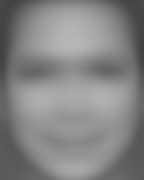
\includegraphics[width=0.6\textwidth]{images/facespace/meanface}
	\end{minipage}
\end{losung*}
Nachdem wir nun das Durchschnittsgesicht gebildet haben, berechnen wir nun die \textit{Differenzgesichter} $\vec a_1,\ldots,\vec a_K$.
Diese sind definiert als
\begin{equation*}
	\vec a_k=\vec b_k-\vec m,\quad k\in\left\{1,\ldots,K\right\}.
\end{equation*}
Die Methode der Eigengesichter trifft nun folgende Annahme:
Die Differenzgesichter sind in guter Approximation in einem niedrig-dimensionalen Unterraum von $\mathbb R^{M\cdot N}$ enthalten.
Wir nennen diesen Unterraum den \textit{Raum der Differenzgesichter} (engl. \textit{facespace}).
Sagen wir, dieser Unterraum habe die Dimension $D\ll M\cdot N$ (\glqq{}viel kleiner als\grqq{}).
Leider können wir das nur stark vereinfacht in für den Fall $M\cdot N=2$ und $D=1$ darstellen.
Dies ist in Abbildung~\ref{fig:meandiff} gezeigt.
\begin{figure}[ht]
	\centering
	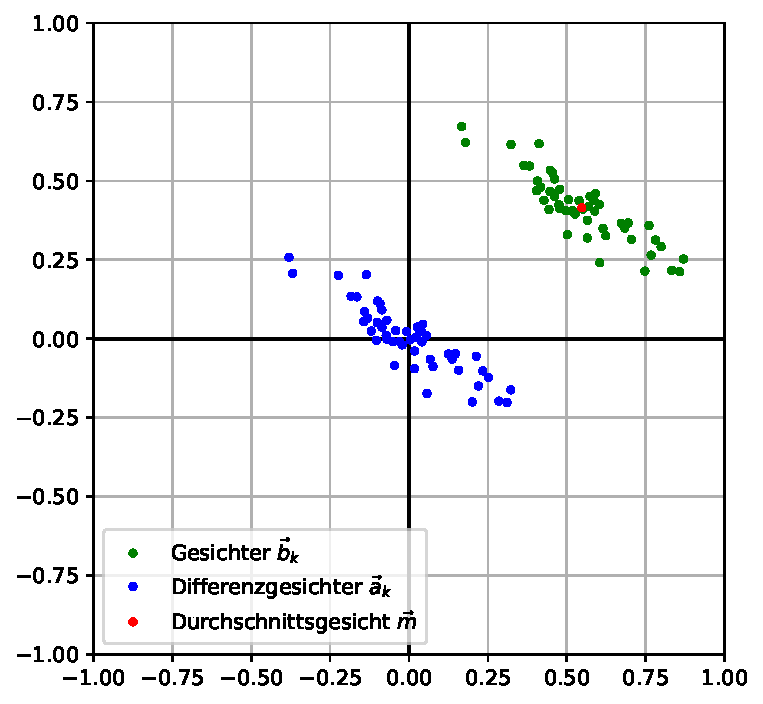
\includegraphics[width=0.5\textwidth]{images/facespace/meandiff}
	\caption{Die Gesichter werden um den Ursprung zentriert indem man das Durchschnittsgesicht subtrahiert.
	Annahme: Die entstehenden Differenzgesichter liegen dann in guter Approximation in einem Unterraum.}
	\label{fig:meandiff}
\end{figure}
\begin{aufgabe}
	Nennen Sie einen Unterschied und eine Gemeinsamkeit der vereinfachten Darstellung in Abbildung~\ref{fig:meandiff} zu unserer tatsächlichen Situation mit Bildern von Gesichtern.
	Gehen Sie davon aus, dass unsere Bilder eine Auflösung von $M=180$ und $N=144$ haben, wie im letzten Kapitel.
\end{aufgabe}
\begin{losung*}
	Als Vektoren aufgefasst sind die Gesichter Punkte im $\mathbb R^{M\cdot N}$.
	Für $M=180$ und $N=144$ wären das Punkte im $\mathbb R^{25'920}$ und nicht im $\mathbb R^2$ wie in der Abbildung.
	Der Unterraum der Differenzgesichter ist zudem dargestellt als Gerade durch Null, also als 1-dimensionaler Raum.
	Wegen der Vielfalt menschlicher Gesichter wird die Dimension tatsächlich viel grösser sein.
	Andererseits wird in der Abbildung korrekt gezeigt, dass die Komponenten der Gesichts-Vektoren $\vec b_k$ nur Werte zwischen 0 und 1 annehmen.
	Zudem sind die Differenzgesichter richtigerweise genau als Verschiebung der Gesichts-Vektoren um $-\vec m$ dargestellt.
\end{losung*}
\subsection{Eigengesichter als Basis}
Im letzten Unterkapitel haben wir den Raum der Differenzgesichter eingeführt.
In diesem Unterkapitel wollen wir eine geeignete Basis dieses Unterraumes finden, nämlich die \textit{Eigengesichter}.
Um uns einige grundlegende Begriffe aus der linearen Algebra in Erinnerung zu rufen, betrachten wir folgende Aufgabe.
\begin{aufgabe}
	Betrachten Sie die Vektoren
	\begin{equation*}
		\vec v_1=\begin{pmatrix}
			\tfrac{3}{5} \\ \tfrac{4}{5} \\ 0
		\end{pmatrix},\quad
		\vec v_2=\begin{pmatrix}
			-\tfrac{4}{5} \\ \tfrac{3}{5} \\  0
		\end{pmatrix},\quad
		\vec v_3=\begin{pmatrix}
			0 \\ 0 \\  1
		\end{pmatrix},\quad
		\vec a=\begin{pmatrix}
			7 \\ 1 \\  4
		\end{pmatrix}.
	\end{equation*}
	\begin{enumerate}[label=(\alph*)]
		\item Die Vektoren $\vec v_1,\vec v_2,\vec v_3$ bilden eine orthonormale Basis von $\mathbb R^3$.
		Begründen Sie warum.
		\item Folglich gibt es genau eine Linearkombination
		\begin{equation*}
			\vec a=c_1\vec v_1+c_2\vec v_2+c_3\vec v_3.
		\end{equation*}
		Berechnen Sie die Koeffizienten $c_1,c_2,c_3$ dieser Linearkombination.
	\end{enumerate}
\end{aufgabe}
\begin{losung*}
	\phantom{text}
	\begin{enumerate}[label=(\alph*)]
		\item Die Vektoren $\vec v_1,\vec v_2,\vec v_3$ sind paarweise orthogonal, also
		\begin{equation*}
			\vec v_1\cdot\vec v_2= \tfrac{3}{5}\cdot\left(-\tfrac{4}{5}\right)+\tfrac{4}{5}\cdot\tfrac{3}{5}+0\cdot 0=0
		\end{equation*}
		und analog findet man $\vec v_1\cdot\vec v_3=0$ und $\vec v_2\cdot\vec v_3=0$.
		Insbesondere sind die Vektoren linear unabhängig.
		Da es drei an der Zahl sind, müssen Sie eine Basis von $\mathbb R^3$ sein.
		Zudem haben die Vektoren Länge Eins, das heisst
		\begin{equation*}
			\vec v_1\cdot\vec v_1= \left(\tfrac{3}{5}\right)^2+\left(\tfrac{4}{5}\right)^2+0^2=1.
		\end{equation*}
		Analog findet man $\vec v_2\cdot\vec v_2=1$ und $\vec v_3\cdot\vec v_3=1$.
		Damit ist diese Basis nicht nur orthogonal, sondern sogar orthonormal.
		\item Da unsere Basis orthonormal ist, kann man die Koeffizienten mit einem Skalarprodukt berechnen.
		Zum Beispiel findet man den Koeffizienten $c_1$ indem man auf beiden Seiten der Gleichung aus der Teilaufgabe das Skalarprodukt mit $v_1$ bildet
		\begin{equation*}
			\vec v_1\cdot\vec a=c_1\underbrace{\vec v_1\cdot\vec v_1}_{=1}+c_2\underbrace{\vec v_1\cdot\vec v_2}_{=0}+c_3\underbrace{\vec v_1\cdot\vec v_3}_{=0},
		\end{equation*}
		also $\vec v_1\cdot\vec a=c_1$.
		Analog erhält man $\vec v_2\cdot\vec a=c_2$ und $\vec v_3\cdot\vec a=c_3$.
		Diese Skalarprodukte berechnen sich zu
		\begin{equation*}
			c_1=5,\quad\quad c_2=-5,\quad\quad c_3=4.
		\end{equation*}
	\end{enumerate}
\end{losung*}

%Die Bilder $\vec a_1,\ldots,\vec a_K$ aus unserer Datenbank sind im Allgemeinen nicht paarweise orthogonal und nicht auf Länge 1 normiert.
Wir werden im Folgenden annehmen, dass die Anzahl der Bilder $K$ viel kleiner ist als die Anzahl der Pixel $M\cdot N$ der einzelnen Bilder.
Der Einfachheit halber nehmen wir zudem an, dass die Vektoren $\vec a_1,\ldots,\vec a_K$ linear unabhängig sind.
Diese bilden dann die Basis eines $K$-dimensionalen Unterraums von $\mathbb R^{M\cdot N}$.
Nun betrachten wir eine weitere Basis dieses Unterraumes, die \textit{Eigengesichter}.
Die Eigengesichter sind eine orthonormale Basis dieses Raumes, wir bezeichnen diese mit $\vec u_1,\dots,\vec u_K\in\mathbb R^{M\cdot N}$.
Diese Basis ist in vielerlei Hinsicht speziell, wie wir sehen werden.
Diese Vektoren können wir wieder als Bilder darstellen.
Das ist in Abbildung~\ref{fig:eigenfaces} gezeigt.
\begin{figure}[ht]
	\centering
	\begin{tabular}{cccccccc}
		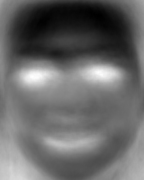
\includegraphics[width=0.1\textwidth]{images/eigenfaces/eigenface00} & 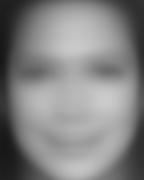
\includegraphics[width=0.1\textwidth]{images/eigenfaces/eigenface01} &
		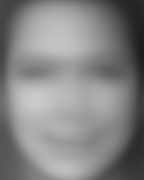
\includegraphics[width=0.1\textwidth]{images/eigenfaces/eigenface02} & 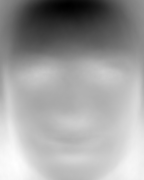
\includegraphics[width=0.1\textwidth]{images/eigenfaces/eigenface03} &
		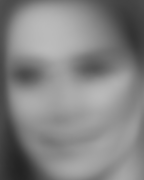
\includegraphics[width=0.1\textwidth]{images/eigenfaces/eigenface04} &
		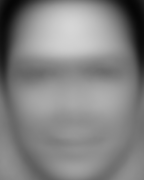
\includegraphics[width=0.1\textwidth]{images/eigenfaces/eigenface05} & 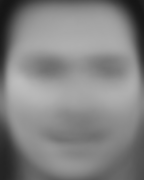
\includegraphics[width=0.1\textwidth]{images/eigenfaces/eigenface06} &
		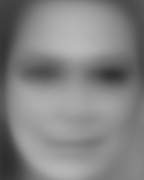
\includegraphics[width=0.1\textwidth]{images/eigenfaces/eigenface07} \\ 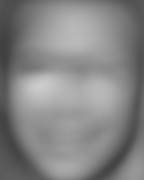
\includegraphics[width=0.1\textwidth]{images/eigenfaces/eigenface08} &
		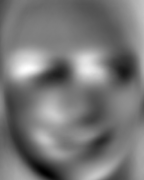
\includegraphics[width=0.1\textwidth]{images/eigenfaces/eigenface09} & 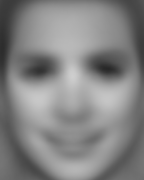
\includegraphics[width=0.1\textwidth]{images/eigenfaces/eigenface10} &
		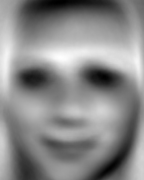
\includegraphics[width=0.1\textwidth]{images/eigenfaces/eigenface11} & 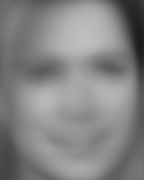
\includegraphics[width=0.1\textwidth]{images/eigenfaces/eigenface12} &
		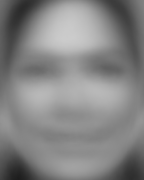
\includegraphics[width=0.1\textwidth]{images/eigenfaces/eigenface13} & 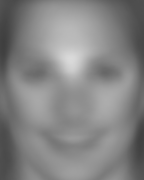
\includegraphics[width=0.1\textwidth]{images/eigenfaces/eigenface14} &
		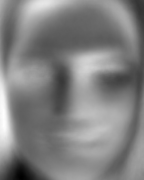
\includegraphics[width=0.1\textwidth]{images/eigenfaces/eigenface15} \\
	\end{tabular}
	\caption{Die ersten 16 Eigengesichter wurden wieder als Bild dargestellt.}
	\label{fig:eigenfaces}
\end{figure}

Wir betrachten nun die Mona Lisa von Leonardo da Vinci, ein Bild das nicht in unserer Datenbank ist.
Um dieses Bild in den Raum der Differenzgesichter zu verschieben, müssen wir noch das Durchschnittsgesicht $\vec m$ subtrahieren.
Das entstehende Differenzgesicht kann dann näherungsweise als Linearkombination der Basis $\vec a_1,\ldots,\vec a_K$ oder auch der Basis der Eigengesichter $\vec u_1,\ldots,\vec u_K$ dargestellt werden.
Letzteres ist in Abbildung~\ref{fig:eigen_basis} dargestellt.
\begin{figure}[ht]
	\centering
	\begin{tabular}{m{1.8cm} c c c c c m{2cm} c c c m{2cm} c c}
		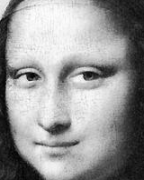
\includegraphics[width=0.1\textwidth]{images/eigenfaces/mona_lisa_original} &
		$-$ & $\vec m$ & $=$ & $c_1$ & $\cdot$ & 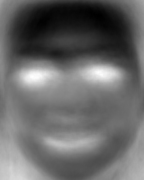
\includegraphics[width=0.1\textwidth]{images/eigenfaces/eigenface00}
		& $+$ & $c_2$ & $\cdot$ & 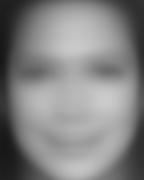
\includegraphics[width=0.1\textwidth]{images/eigenfaces/eigenface01} & $+$ & $\cdots$
	\end{tabular}
	\caption{Differenzgesicht der Mona Lisa als Linearkombination der Eigengesichter.}
	\label{fig:eigen_basis}
\end{figure}
\begin{aufgabe}
	Sei $\vec p\in\mathbb R^{M\cdot N}$ das Bild der Mona Lisa und $\vec u_1,\ldots,\vec u_K\in\mathbb R^{M\cdot N}$ die Eigengesichter.
	Berechnen Sie die Koeffizienten $c_1,\ldots,c_K$ der Linearkombination der Eigengesichter, also
	\begin{equation*}
		\vec p-\vec m=c_1\vec u_1+c_2\vec u_2+\ldots+c_K\vec u_K
	\end{equation*}
	wie in Abbildung~\ref{fig:eigen_basis} gezeigt.
	Das heisst, geben Sie die Koeffizienten in Termen von $\vec p, \vec m$ und den Eigengesichtern an.
\end{aufgabe}
\begin{losung*}
	Wie in der letzten Aufgabe verwenden wir, das die Eigengesichter orthonormal sind.
	Wir bilden das Skalarprodukt beider Seiten der obigen Gleichung mit $u_1$, also
	\begin{equation*}
		\vec u_1\cdot\left(\vec p-\vec m\right)=c_1\underbrace{\vec u_1\cdot\vec u_1}_{=1}+c_2\underbrace{\vec u_1\cdot\vec u_2}_{=0}+\ldots+c_K\underbrace{\vec u_1\cdot\vec u_K}_{=0}.
	\end{equation*}
	Wenn wir das auch noch mit $\vec u_2,\ldots,\vec u_K$ machen erhalten wir
	\begin{equation*}
		\vec u_k\cdot\left(\vec p-\vec m\right)=c_k,
	\end{equation*}
	für alle $k\in\{1,\ldots,K\}$.
\end{losung*}
Hat man die Koeffizienten der Linearkombination berechnet, so kann das Bild $\vec p$ der Mona Lisa wieder als Linearkombination der Eigengesichter darstellen
\begin{equation*}
	\vec p=\vec m+c_1\vec u_1+c_2\vec u_2+\ldots+c_Ku_K.
\end{equation*}
Das werden wir in der nächsten Aufgabe implementieren.
\begin{aufgabe} \label{aufg:compute_coefficients}
	Seien \texttt{p} und \texttt{m} Vektoren der Länge $M\cdot N$, wobei \texttt{p} ein Gesicht zeigt (z.B. das der Mona Lisa) und \texttt{m} das Durchschnittsgesicht ist.
	Sei zudem \texttt{u\_list} die Liste der Eigengesichter als Vektoren.
	Ergänzen Sie die Funktion \texttt{compute\_coefficients(p, m, u\_list)}, welche die Liste der Koeffizienten der Linearkombination aus Abbildung~\ref{fig:eigen_basis} zurück gibt.
	Um Ihre Lösung zu testen können Sie das Python Skript \texttt{basis\_expansion.py} laufen lassen, welches das Bild der Mona Lisa mit ihren Koeffizienten rekonstruiert.
	\textit{Hinweis:} Mit \texttt{np.dot(v,w)} lässt sich das Skalarprodukt zweier Vektoren \texttt{v} und \texttt{w} berechnen.
\end{aufgabe}
\begin{losung*}
	Die Lösung könnte zum Beispiel so aussehen.\\[0.5cm]
	\begin{minipage}{0.65\textwidth}
\begin{lstlisting}[style=python]
import numpy as np

def compute_coefficients(p, m, u_list):
	K = len(u_list)
	c_list = np.empty((K,))
	for c, u in zip(c_list, u_list):
		c = np.dot(u, p - m)
	return c_list
\end{lstlisting}
	\end{minipage}\hfill
	\begin{minipage}{0.35\textwidth}\vspace{-1cm}
		\centering Rekonstruktion:\\[0.5cm]
		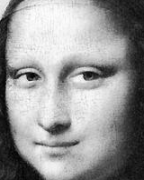
\includegraphics[width=0.4\textwidth]{images/eigenfaces/mona_lisa_original}
	\end{minipage}
\end{losung*}
Wir haben die Eigengesichter einfach als eine spezielle orthonormale Basis des Raumes der Differenzgesichter eingeführt.
Tatsächlich sind sie aber nicht etwa eine fixe Basis, sonder sie werden aus den Bilder der Datenbank berechnet.
Insbesondere erhält man mit einer anderen Datenbank auch andere Eigengesichter.
Aber wie diese Berechnung das genau geht, sehen wir später.
Zuerst wollen wir einige Eigenschaften dieser Basis untersuchen.
\subsection{Bildkompression}
Wenn wir ein schwarz-weiss Bild mit der Auflösung $M=144$ mal $N=180$ Pixel für Pixel abspeichern, so müssen wir $M\cdot N=25920$ Zahlen abspeichern.
Unter Bildkompression versteht man Verfahren, die Bilder mit weniger Zahlen darstellen können.
Das ist zum Beispiel nützlich wenn man Bilder über das Internet verschicken möchte (oder gleich ganze Filme).
Die Datenmenge kann durch Kompression stark verringert werden, was zu viel kürzeren Download-Zeiten führt.
Mit den Eigengesichtern lassen sich Bilder von Gesichtern komprimieren.
Grund dafür ist eine spezielle Eigenschaft, welche die Eigengesichter auszeichnet, und dir wir nun untersuchen werden.

Im letzten Kapitel haben wir das Gemälde der Mona Lisa als Linearkombination der Eigengesichter geschrieben.
Dazu mussten wir mit geeigneten Skalarprodukten die Koeffizienten $c_1,\ldots,c_K$ dieser Linearkombination berechnen.
Allerdings bilden (gemäss unserer Annahme aus dem letzten Kapitel) die Differenzbilder der Bilder aus der Datenbank, also $\vec a_1,\ldots,\vec a_K$, auch eine Basis des Raumes der Differenzgesichter.
Wir hätten also das Bilder der Mona Lisa auch als Linearkombination dieser Basis darstellen können, was in Abbildung~\ref{fig:mona_lisa_reconstruction} gezeigt ist.
\begin{figure}[ht]
	\centering
	\begin{tabular}{lcr}
		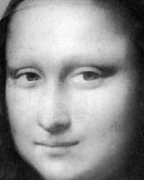
\includegraphics[width=0.2\textwidth]{images/eigenfaces/mona_lisa_naive_approx} &
		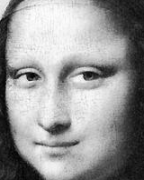
\includegraphics[width=0.2\textwidth]{images/eigenfaces/mona_lisa_original} & 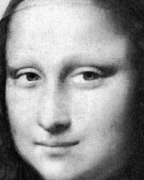
\includegraphics[width=0.2\textwidth]{images/eigenfaces/mona_lisa_eigen_approx}
	\end{tabular}
	\caption{Rekonstruktion der Mona Lisa als Linearkombination der $\vec a_1,\ldots,\vec a_K$ (links) und der Eigengesichter $\vec u_1,\ldots,\vec u_K$ (rechts). In der Mitte ist das Original.}
	\label{fig:mona_lisa_reconstruction}
\end{figure}
Ein wesentlicher Unterschied zwischen diesen beiden Basen ist die Verteilung der Beträge der Koeffizienten, also $\lvert c_1\rvert,\ldots,\lvert c_K\rvert$.
Diese sind in Abbildung~\ref{fig:coef} gezeigt.
\begin{figure}[ht]
	\centering
	\begin{tabular}{lr}
		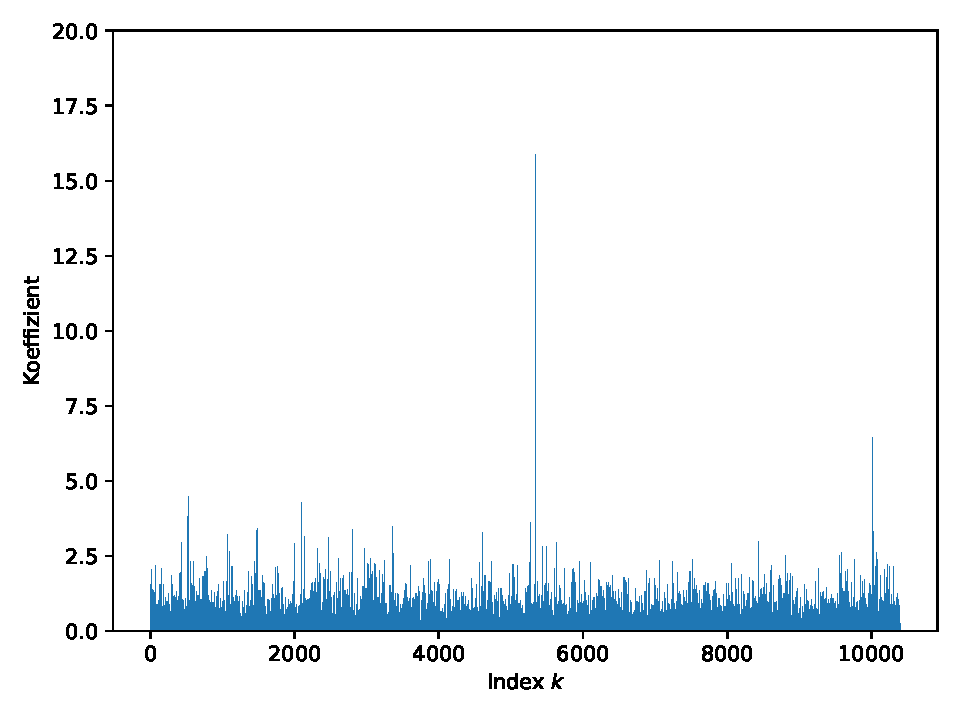
\includegraphics[width=0.45\textwidth]{images/eigenfaces/naive_coef} & 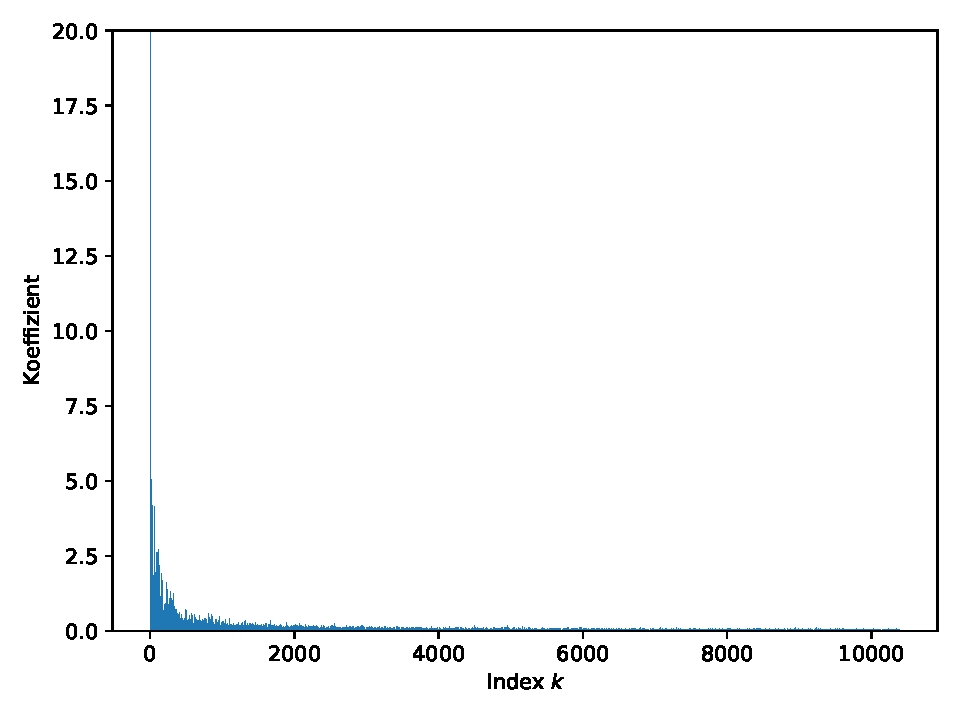
\includegraphics[width=0.45\textwidth]{images/eigenfaces/eigen_coef} \\
	\end{tabular}
	\caption{Der Absolutbetrag der Koeffizienten der Linearkombination des Differenzgesichtes der Mona Lisa. Links wurden als Basis die Differenzgesichter der Datenbank und rechts die Eigengesichter genommen.}
	\label{fig:coef}
\end{figure}
\begin{aufgabe}
	Betrachten Sie die Abbildung~\ref{fig:coef}, welche die Koeffizienten der Linearkombinationen bezüglich der beiden Basen zeigt.
	Beschreiben Sie die Unterschiede der Bilder.
	Welche Rückschlüsse kann man dadurch auf die entsprechenden Basen ziehen?
\end{aufgabe}
\begin{losung*}
	Die Koeffizienten der Eigengesichter fallen schnell ab.
	Dem rechten Bild kann man entnehmen, dass ungefähr die ersten 2000 Eigengesichter fast den ganzen Beitrag zur Linearkombination leisten.
	Bei der Basis der Differenzgesichter ist keine solche Struktur zu erkennen.
	In diesem Sinn sind alle diese Differenzgesichter etwa gleich wichtig um das Bild der Mona Lisa darstellen zu können.
\end{losung*}
Was wir hier in Abbildung~\ref{fig:coef} beobachtet haben ist kein Einzelfall.
Obwohl wir nur das Beispiel der Mona Lisa betrachtet haben, würden andere Gesichter ähnlich verteilte Koeffizienten liefern.
Die Lösung der vorherigen Aufgabe ist zugleich die Grundidee der Bildkompression mittels Eigengesichter.
Anstatt alle der $K$ Eigengesichter, verwenedt man nur die ersten $\tilde K$ Eigengesichter um ein Bild darzustellen.
Die Abbildung~\ref{fig:coef} lässt vermuten, dass wenn $\tilde K$ gross genug gewählt ist, aber immer noch viel kleiner als $K$, dann sollte das nicht viel an der Bildqualität ändern.
Genauer gesagt, können wir ablesen, dass wohl die ersten $\tilde K=2000$ Eigengesichter ausreichend sein sollten.
Nun wollen ein Bild $\vec p$ rekonstruieren, indem wir nur die ersten $\tilde K$ Eigengesichter verwenden.
Das rekonstruierte Gesicht bezeichnen wir mit $\vec p_{\tilde K}$, also
\begin{equation*}
	\vec p_{\tilde K}=\vec m+c_1\vec u_1+c_2\vec u_2+\ldots+c_{\tilde K}\vec u_{\tilde K},
\end{equation*}
wobei $\tilde K\leq K$ und $\vec u_1,\ldots,\vec u_{\tilde K}$ sind die ersten $\tilde K$ Eigengesichter.
Wie man die Koeffizienten $c_1,\ldots,c_{\tilde K}$ berechnet, haben wir im letzten Kapitel gesehen.
\begin{aufgabe}
	Ergänzen Sie die Funktion \texttt{compress(p, m, u\_list, K\_tilde)}, welche einen Vektor der Länge $M\cdot N$ zurück gibt, der dem Bild $\vec p_{\tilde K}$ entspricht.
	Hier bezeichnen \texttt{p} das ursprüngliche Bild $\vec p$ und \texttt{m} das Durchschnittsgesicht $\vec m$.
	Die Liste \texttt{u\_list} enthält die Eigengesichter und \texttt{K\_tilde} entspricht der Anzahl $\tilde K$ der Eigengesichter, die verwendet werden sollen.
	Testen Sie ihre Lösung indem Sie das Skript \texttt{compress.py} laufen lassen, welches die rekonstruierten Bilder ausgibt.
	\textit{Hinweis:} Verwenden Sie in ihrem Code die Funktion \texttt{compute\_coefficients(p, m, u\_list)} aus Aufgabe~\ref{aufg:compute_coefficients}.
\end{aufgabe}
\begin{losung*}
	Die Lösung könnte zum Beispiel so aussehen.
\begin{lstlisting}[style=python]
import numpy as np

def compress(p, m, u_list, K_tilde):
	# Reduzierte Liste der ersten K_tilde Eigengesichter
	u_list_reduced = u_list[:K_tilde]
	c_list_reduced = compute_coefficients(p, m, u_list_tilde)
	p_tilde = np.dot(u_list_reduced, c_list_reduced)
	return p_tilde
\end{lstlisting}
Die durch \texttt{compress.py} generierten Bilder sind in Abbildung~\ref{fig:compression} gezeigt.
\end{losung*}
\begin{figure}[ht]
	\centering
	\begin{tabular}{cccc}
		$\tilde K=20$ & $\tilde K=500$ & $\tilde K=2000$ & original \\
		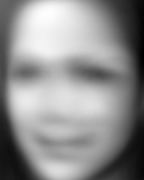
\includegraphics[width=0.1\textwidth]{images/compression/mona_lisa_20} &
		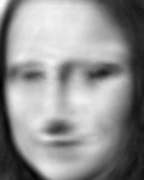
\includegraphics[width=0.1\textwidth]{images/compression/mona_lisa_200} &
		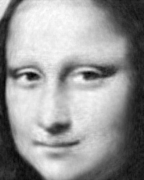
\includegraphics[width=0.1\textwidth]{images/compression/mona_lisa_2000} & 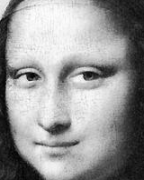
\includegraphics[width=0.1\textwidth]{images/compression/mona_lisa} \\
		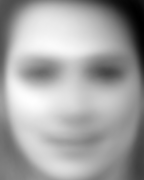
\includegraphics[width=0.1\textwidth]{images/compression/queen_elizabeth_20} &
		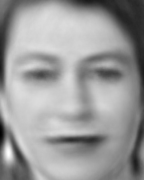
\includegraphics[width=0.1\textwidth]{images/compression/queen_elizabeth_200} &
		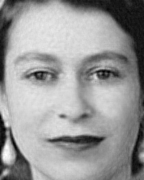
\includegraphics[width=0.1\textwidth]{images/compression/queen_elizabeth_2000} & 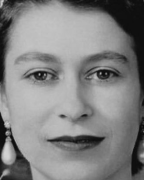
\includegraphics[width=0.1\textwidth]{images/compression/queen_elizabeth} \\
		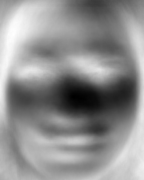
\includegraphics[width=0.1\textwidth]{images/compression/chair_20} &
		\includegraphics[width=0.1\textwidth]{images/compression/chair_200} &
		\includegraphics[width=0.1\textwidth]{images/compression/chair_2000} & \includegraphics[width=0.1\textwidth]{images/compression/chair} \\
		\includegraphics[width=0.1\textwidth]{images/compression/columbia_20} &
		\includegraphics[width=0.1\textwidth]{images/compression/columbia_200} &
		\includegraphics[width=0.1\textwidth]{images/compression/columbia_2000} & \includegraphics[width=0.1\textwidth]{images/compression/columbia}
	\end{tabular}
	\caption{Rekonstruktion mit verschiedenen $\tilde K$. Gezeigt sind die Mona Lisa, Queen Elizabeth, ein Stuhl und das erste Space Shuttle \glqq{}Columbia\grqq{}. Gesichter werden generell besser rekonstruiert als andere Bilder.}
	\label{fig:compression}
\end{figure}
Was wir in Abbildung~\ref{fig:compression} beobachten ist eine Bildkompression.
Sind die Eigengesichter bekannt, so lässt sich ein Bild rekonstruieren aus den Koeffizienten $c_1,\ldots,c_{\tilde K}$ der ersten $\tilde K$ Eigengesichter.
Um ein Bild eines Gesichtes in leicht verminderter Qualität über das Internet zu versenden, wäre es ausreichend, nur $\tilde K=2000$ Zahlen zu versenden, sofern der Empfänger über die Eigengesichter verfügt.
Wir erinnern uns, dass ein Bild welches Pixelweise versendet wird, $M\cdot N=25920$ Zahlen benötigt.
Das ist etwa ein Faktor 13 mehr als die komprimierte Variante.
Trotzdem sieht man für $\tilde K=2000$ kaum einen Unterschied zum Original in Abbildung~\ref{fig:compression}.
Gleichzeitig sehen wir, dass die aggressivere Komprimierung mit $\tilde K=200$ die Bildqualität doch sehr vermindert.
Aber das konnte man aufgrund des rechten Verteilung in Abbildung~\ref{fig:coef} schon vermuten.
Die linke Verteilung zeigt zugleich, dass dies mit der Basis der Differenzgesichter nicht möglich gewesen wäre.
Weiter beobachten wir, dass die Komprimierung für Bilder, welche kein Gesicht zeigen, weniger gut funktioniert.
Der Grund dafür ist, das andere Differenzbilder nicht notwendigerweise nahe am Raum der Differenzgesichter liegen.
Doch die Eigengesichter sind eine Basis eben dieses Unterraumes.
\section{Gesichtserkennung} \label{sec:recognition}
\begin{tcolorbox}
	\centerline{\textbf{Lernziele Kapitel~\ref{sec:recognition}}}
	\begin{enumerate}[leftmargin=*,label=\thesection.\arabic*]
		\item \textit{Erklären} können, was eine Klassifizierung ist.
		\item \textit{Erklären} können, warum eine Gesichtserkennung ein Klassifizerungsproblem ist.
		\item \textit{Verstehen} wie die Eigengesichter das \glqq{}Ähnlich aussehen\grqq{} von Gesichtern quantifizieren können.
	\end{enumerate}
\end{tcolorbox}
Nun wollen wir die Eigengesichter nutzen für eine Gesichtserkennung nutzen.
Wie bereits in der Einleitung erklärt, ist Gesichtserkennung im Grunde eine Klassifizierung.
Hier als Beispiel betrachten wir 8 verschiedene Klassen.
\begin{table}[ht]
	\centering
	\begin{tabular}{|c|c|c|c|}
		\hline
		Daniel Radcliffe & Emma Stone & Emma Watson & Eva Green \\
		\includegraphics[width=0.2\textwidth]{images/recognition/Daniel_Radcliffe} & \includegraphics[width=0.2\textwidth]{images/recognition/Emma_Stone} & \includegraphics[width=0.2\textwidth]{images/recognition/Emma_Watson} & \includegraphics[width=0.2\textwidth]{images/recognition/Eva_Green} \\ \hline
		Jennifer Lawrence & Orlando Bloom & Pierce Brosnan & Tom Cruise \\
		\includegraphics[width=0.2\textwidth]{images/recognition/Jennifer_Lawrence} & \includegraphics[width=0.2\textwidth]{images/recognition/Orlando_Bloom} & \includegraphics[width=0.2\textwidth]{images/recognition/Pierce_Brosnan} & \includegraphics[width=0.2\textwidth]{images/recognition/Tom_Cruise} \\ \hline
	\end{tabular}
	\caption{Die acht verschiedenen Klassen. }
	\label{tab:classes}
\end{table}
Wir verwenden in diesem Kapitel eine Datenbank die nur aus Bilder dieser 8 Personen besteht.
Dabei enthält sie von jeder Person genau 10 Bilder.
Das heisst, sie besteht aus $K=8\cdot 10=80$ Bildern.
Pro Klasse haben wir zusätzlich 3 Testbilder.
Das sind Bilder die zwar jeweils eine dieser 8 Personen zeigen, aber nicht in der Datenbank enthalten sind.
Das Ziel ist nun die Testbilder möglichst der richtigen Klasse zuzuordnen.
So können wir unsere Gesichtserkennung testen, daher der Name \glqq{}Testbilder\grqq{}.
\begin{figure}[ht]
	\centering
	\begin{tabular}{|c m{2cm} m{2cm} m{2cm} m{2cm} m{2cm}|}
		\hline
		Datanbank &
		\includegraphics[width=0.1\textwidth]{images/recognition/training_faces/training_0} &
		\includegraphics[width=0.1\textwidth]{images/recognition/training_faces/training_1} &
		\includegraphics[width=0.1\textwidth]{images/recognition/training_faces/training_2} &
		\includegraphics[width=0.1\textwidth]{images/recognition/training_faces/training_3} &
		\includegraphics[width=0.1\textwidth]{images/recognition/training_faces/training_4} \\
		&
		\includegraphics[width=0.1\textwidth]{images/recognition/training_faces/training_5} &
		\includegraphics[width=0.1\textwidth]{images/recognition/training_faces/training_6} &
		\includegraphics[width=0.1\textwidth]{images/recognition/training_faces/training_7} &
		\includegraphics[width=0.1\textwidth]{images/recognition/training_faces/training_8} &
		\includegraphics[width=0.1\textwidth]{images/recognition/training_faces/training_9} \\ \hline
		Testbilder &
		\includegraphics[width=0.1\textwidth]{images/recognition/test_faces/test_0} &
		\includegraphics[width=0.1\textwidth]{images/recognition/test_faces/test_1} &
		\includegraphics[width=0.1\textwidth]{images/recognition/test_faces/test_2} &
		& \\ \hline
	\end{tabular}
	\caption{Datenbank- und Testbilder am Beispiel der Klasse \glqq{}Daniel Radcliffe\grqq{}}
	\label{fig:testfaces}
\end{figure}
Zwar ist das für einen Menschen ganz leicht, aber für einen Computer ist das überhaupt nicht einfach.
Im Grunde müssen wir den Computer lehren, wann zwei Bilder ähnlich aussehen.
Dazu brauchen wir ein Mass für die Distanz zweier Bilder.
Es stellt sich heraus, dass die Eigengesichter ein Solches liefern.
Seien nun $\vec p$ und $\vec q$ zwei Bilder von Gesichtern.
Wir schreiben die entsprechenden Differenzgesichter als Linearkombination der Eigengesichter
\begin{equation*}
	\vec p-\vec m=c_1\vec u_1+c_2\vec u_2+\ldots+c_K\vec u_K
\end{equation*}
und
\begin{equation*}
	\vec q-\vec m=\tilde c_1\vec u_1+\tilde c_2\vec u_2+\ldots+\tilde c_K\vec u_K,
\end{equation*}
wobei nun $K=80$ und $\vec m$ das Durchschnittsgesicht der Bilder der neuen Datenbank ist.
Entsprechend sehen die Eigengesichter auch etwas anders aus, aber deren Eigenschaften sind die selben.
Das besagte Mass der Distanz zwischen den Gesichtern $\vec p$ und $\vec q$ definieren wir als
\begin{equation*}
	D\left(\vec p,\vec q\right)=\left(c_1-\tilde c_1\right)^2+\left(c_2-\tilde c_2\right)^2+\ldots+\left(c_K-\tilde c_K\right)^2.
\end{equation*}
\begin{aufgabe}
	Warum entspricht dieser Begriff von Distanz dem \glqq{}Ähnlich aussehen\grqq{} von Gesichtern?
	Erklären Sie in Worten.
	\textit{Hinweis:} Rufen Sie sich die Konstruktion der Eigengesichter und die Diskussion am Ende von Kapitel~\ref{sec:facespace} in Erinnerung.
\end{aufgabe}
\begin{losung*}
	Die Eigengesichter fangen gewisse Gesichtszüge ein.
	Die Funktion $D\left(\vec p,\vec q\right)$ vergleicht, wie fest sich $\vec p$ und $\vec q$ in eben diesen Gesichtszügen unterscheiden.
	Dabei werden die ersten Eigengesichter am stärksten gewichtet, da ihre Koeffizienten typischerweise am grössten sind (Abbildung~\ref{fig:coef}).
	Das macht auch Sinn, denn es sind genau die ersten Eigengesichter (Gesichtszüge), in denen sich die Gesichter der Datenbank am meisten unterscheiden.
	Die Bilder nur Pixel für Pixel zu vergleichen macht keinen Sinn, denn kein Pixel kann alleine eine Information über ein Gesicht tragen.
	Anders gesagt können sich zwei Bilder in jedem Pixel stark unterscheiden und dennoch die selbe Person zeigen.
	Mit Gesichtszügen ist dies kaum möglich.
\end{losung*}
Sei nun ein Bild $\vec p\in\mathbb R^{M\cdot N}$ gegeben.
Wir wissen über das Bild, dass es eine der 8 Personen aus Tabelle~\ref{tab:classes} zeigt.
Jedoch wissen wir nicht welche.
Doch wir werden versuchen das mit folgendem Verfahren zu erraten.
\begin{enumerate}[leftmargin=3cm, label=Schritt \arabic*:]
	\item Seien $\vec q_1,\ldots,\vec q_{80}\in\mathbb R^{M\cdot N}$ die Bilder der Datenbank.
	Wir berechnen die Distanz $D\left(\vec p,\vec q_i\right)$ für alle $i\in\left\{1,\ldots,80\right\}$.
	\item Eines dieser Bilder wird die kleinste Distanz zu $\vec p$ haben, sagen wir das ist $\vec q_j$ für ein bestimmtes $j\in\left\{1,\ldots,80\right\}$.
	\item Wir schauen in der Datenbank nach, welche Person auf dem Bild $\vec q_j$ gezeigt ist. Da $\vec p$ ähnlich aussieht, zeigt es wohl die selbe Person und wir klassifizieren $\vec p$ entsprechend.
\end{enumerate}
\begin{aufgabe}
	Ergänzen sie die Funktion \texttt{D(p,q)} welche die Distanz $D\left(\vec p,\vec q\right)$ zweier Bilder zurück gibt.
	Dabei entsprechen \texttt{p} und \texttt{q} den Vektoren $\vec p$ und $\vec q$.
\end{aufgabe}
%\section{Berechnung der Eigengesichter: Singulärwertzerlegung}
Wir betrachten die Matrix, deren Spalten aus den Bildern der Datenbank bestehen, also
\begin{equation*}
	A=\left(\vec a_1,\ldots,\vec a_K\right).
\end{equation*}
Wenn wir diese Matrix auf einen Vektor $\vec c\in\mathbb R^K$ anwenden, dann berechnet diese gerade die Linearkombination der Bilder $\vec a_1,\ldots,\vec a_K$ und die Komponenten von $\vec c$ sind gerade die Koeffizienten dieser Linearkombination
\begin{equation*}
	Ac=c_1\vec a_1+\ldots+c_K\vec a_K.
\end{equation*}
Der Vektor $A\vec c$ liegt wieder in $\mathbb R^{M\cdot N}$ und kann als Bild interpretiert werden, falls dessen Einträge in $\left[0,1\right]$ liegen.
In diesem Sinne ist $A\vec c$ eine gewichtete Überlagerung der Bilder/Gesichter der Datenbank und liegt $A\vec c$ im Raum der Differenzgesichter.
\begin{aufgabe}
	Welches Format hat die Matrix $A$, d.h. wie viele Zeilen und Spalten hat sie?
	Geben sie dies durch die Variablen $K,M$ und $N$ an. 
\end{aufgabe}
\begin{losung*}
	Sie hat das Format $\left(M\cdot N\right)\times K$.
	Das heisst sie hat $M\cdot N$ Zeilen (eine für jedes Pixel) und $K$ Spalten (eine für jedes Bild in der Datenbank).
\end{losung*}
Nun verwenden wir (ohne Herleitung) ein klassisches Resultat aus der linearen Algebra, die \textit{Singulärwertzerlegung}.
Zudem nehmen wir an, dass $K\leq M\cdot N$, also dass die Anzahl der Bilder der Datenbank kleiner oder gleicher der Anzahl Pixel eines Bildes ist.
In diesem Fall besitzt die Matrix $A$ besitzt eine Zerlegung der Form
\begin{equation*}
	A=U\Sigma V^T,
\end{equation*}
wobei $U\in\mathbb R^{\left(M\cdot N\right)\times K},V\in\mathbb R^{\left(M\cdot N\right)\times K}$ und $\Sigma\in\mathbb R^{K\times K}$ Matrizen sind, mit folgenden Eigenschaften:
\begin{itemize}
	\item Die Spalten $u_1,\ldots,u_K\in\mathbb R^{M\cdot N}$ der Matrix $U$ sind orthonormal.
	\item Die Spalten $v_1,\ldots,v_K\in\mathbb R^{M\cdot N}$ der Matrix $V$ sind orthonormal.
	\item Die Matrix $\Sigma$ ist diagonal mit den Einträgen $\sigma_1\geq\ldots\geq\sigma_K\geq 0$.
	Diese Diagonal-Einträge heissen \textit{Singulärwerte} von $A$.
\end{itemize}
Eine Zerlegung dieser Form heisst Singulärwertzerlegung.
Schematisch kann man das auch folgendermassen darstellen
\begin{equation}\label{eq:svd}
A=
\begin{pmatrix}
	\vert & \vert & \cdots & \vert \\
	u_1   & u_2   & \cdots & u_K \\
	\vert & \vert & \cdots & \vert
\end{pmatrix}
\,
\begin{pmatrix}
	\sigma_1 & & & \\
	& \sigma_2 & & \\
	& & \ddots & \\
	& & & \sigma_K
\end{pmatrix}
\,
\begin{pmatrix}
	\text{---} & v_1^T & \text{---} \\
	\text{---} & v_2^T & \text{---} \\
	\vdots & \vdots & \vdots \\
	\text{---} & v_K^T & \text{---}
\end{pmatrix}.
\end{equation}
Wir haben vorher gesehen, dass die Matrix-Vektor Multiplikation $Ac$ eigentlich eine Linearkombination der Spaltenvektoren von $A$ bildet und diese Spalten sind genau die Bilder aus der Datenbank.
Doch über die Singulärwertzerlegung können wir den Vektor $Ac$ auch als Linearkombination der Spaltenvektoren $u_1,\ldots,u_K$ von $U$ interpretieren.
Dazu ersetzen wir im Term $Ac$ die Matrix $A$ durch ihre Singulärwertzerlegung in Gleichung~\ref{eq:svd}.
Dann berechnen wir die Matrix-Vektor Multiplikationen von rechts nach links.
Das heisst wir beginnen mit $V^Tc$, also
\begin{equation*}
	V^Tc=
	\begin{pmatrix}
		\text{---} & v_1^T & \text{---} \\
		\text{---} & v_2^T & \text{---} \\
		\vdots & \vdots & \vdots \\
		\text{---} & v_K^T & \text{---}
	\end{pmatrix}
	\begin{pmatrix}
		c_1 \\
		c_2 \\
		\vdots \\
		c_{M\cdot N}
	\end{pmatrix}=
	\begin{pmatrix}
		v_1^T c \\
		v_2^T c \\
		\vdots \\
		v_K^T c
	\end{pmatrix}.
\end{equation*}
Die Komponenten des Vektors $V^Tc$ sind also die Skalarprodukte der $v_k$ mit $c$.
Folglich gilt
\begin{equation*}
	\Sigma V^Tc=
	\begin{pmatrix}
		\sigma_1 & & & \\
		& \sigma_2 & & \\
		& & \ddots & \\
		& & & \sigma_K
	\end{pmatrix}\,
	\begin{pmatrix}
		v_1^T c \\
		v_2^T c \\
		\vdots \\
		v_K^T c
	\end{pmatrix}=
	\begin{pmatrix}
		\sigma_1 v_1^T c \\
		\sigma_2 v_2^T c \\
		\vdots \\
		\sigma_K v_K^T c
	\end{pmatrix}.
\end{equation*}
Wenn wir den Vektor auf der rechten Seite mit $\tilde c$ bezeichnen, also $\tilde c_k=\sigma_k v_k^T c$, dann erhalten wir schliesslich
\begin{equation*}
	Ac = U\Sigma V^Tc=U\tilde c
	=\tilde c_1 u_1+\ldots+\tilde c_K u_K.
\end{equation*}
Hier sehen wir bereits, dass das $Ac$ eine Linearkombination der Vektoren $u_1,\ldots,u_K$ ist.
Wenn wir für $\tilde c_k$ wieder $\sigma_k v_k^T c$ ersetzen, können wir das noch ausschreiben als
\begin{equation}\label{eq:span_uk}
	Ac =\left(\sigma_1 v_1^Tc\right) u_1+\ldots+\left(\sigma_K v_K^Tc\right) u_K.
\end{equation}
\begin{aufgabe}
	Gleichung~\eqref{eq:span_uk} sagt, dass jede Linearkombination von Bildern aus der Datenbank $a_1,\ldots,a_K$ auch als Linearkombination der Spalten $u_1,\ldots,u_K$ von $U$ geschrieben werden kann.
	Erklären Sie, warum das so ist.
\end{aufgabe}
\begin{losung*}
	Wir haben gesehen, dass für jeden Vektor $c\in\mathbb R^K$ die Matrix-Vektor Multiplikation $Ac$ gerade die Linearkombination
	\begin{equation*}
		c_1u_1+\ldots+c_Ku_K
	\end{equation*}
	der Spalten von $A$ bildet.
	Durch Variation von $c$ kann so jede mögliche Linearkombination der Bilder aus der Datenbank generiert werden.
	Doch zu jeder solcher Linearkombination liefert Gleichung~\eqref{eq:span_uk} eine entsprechende Linearkombination der $u_1,\ldots,u_K$ die den gleichen Vektor darstellt.
\end{losung*}
\begin{aufgabe}
	Sei $k\in\left\{1,\ldots,K\right\}$ beliebig.
	Schreiben Sie das $k$-te Bild aus der Datenbank, also $a_k$, also Linearkombination der $u_1,\ldots,u_K$.
	Das heisst, geben Sie die Koeffizienten dieser Linearkombination an in Termen von $\sigma_1,\ldots,\sigma_K$ und $v_1,\dots,v_K$.
\end{aufgabe}
\begin{losung*}
	Wir wählen in Gleichung~\ref{eq:span_uk} den Vektor $c$ so, dass $Ac$ genau das Gesicht $a_k$ ausliest.
	Dazu müssen alle Komponenten von $c$ Null sein, ausser die $k$-te Komponente ist Eins, also
	\begin{equation*}
		c^T=\left(0\ \ldots\ 0\ \smash{\overbrace{1}^{k\textrm{-te Komponente}}}\ 0\ \ldots\ 0\right).
	\end{equation*}
	Nun gilt $a_k=Ac$.
	Mit dieser Wahl von $c$ liefert Gleichung~\eqref{eq:span_uk} die gewünschte Linearkombination
	\begin{equation*}
		a_k=\left(\sigma_1 v_1^Tc\right) u_1+\ldots+\left(\sigma_K v_K^Tc\right) u_K.
	\end{equation*}
\end{losung*}

\begin{tcolorbox}
	\centerline{\textbf{Lernzielkontrolle Kapitel 1}}
	\begin{aufgabe}
		Frage zu Lernziel 1 folgt...
	\end{aufgabe}
	\begin{aufgabe}
		Frage zu Lernziel 2 folgt...
	\end{aufgabe}
	\begin{aufgabe}
		Frage zu Lernziel 3 folgt...
	\end{aufgabe}
	\begin{aufgabe}
		Frage zu Lernziel 4 folgt...
	\end{aufgabe}
\end{tcolorbox}

\subsection{Didaktische Methoden}
\begin{itemize}
	\item interleaved practice: Anstatt zuerst die ganze Theorie zu entwickeln und anschliessend zu programmieren, wechseln die Aufgaben ab: Es kommen abwechslungsweise Theorie- und Programmieraufgaben.
	Diese \textit{interleaved practice} verspricht langfristig besseren Lernerfolg verglichen mit der sequenziellen Alternative \cite{Rohrer14}.
	\item Unterteilung der Lernziele nach der revidierten Taxonomie von Bloom \cite{Anderson2001}.
	\item ...
\end{itemize}
\nocite{*}
\bibliographystyle{plain}
\bibliography{references}
\end{document}